\documentclass[english, DIV=13]{scrartcl}

% Packages
\usepackage{pgfplots}
\usepackage{amsmath}
\usepackage{empheq}
\usepackage{hyperref}
\usepackage{todonotes}

\renewcommand{\vec}[1]{\mathbf{#1}}

\title{LINMA1731 - Project}
\author{Antoine Paris\and Matthieu Xhonneux}
\date{\today}

\begin{document}
\maketitle

\section{Discrete-time version of the Lorenz system}
The Lorenz dynamical system is given by
\begin{equation*}
    \begin{cases}
        \dot{x} &= a(y-x) \\
        \dot{y} &= x(r-z) \\
        \dot{z} &= xy - bz
    \end{cases}.
\end{equation*}
Using first-order forward finite difference, that is approximating $\dot{x}(t)$ by
\[ \frac{x(t+\delta t) - x(t)}{\delta t} := \frac{x_{k+1} - x_k}{\delta t}, \]
a discrete-time version of the form
\[ \vec{x}_{k+1} = F(\vec{x}_k) + \Gamma\vec{u}_k \]
can be obtained. In this case, the function $F$ is given by
\begin{equation*}
    \begin{cases}
        F_1(\vec{x}_k) &= ay_k\delta t + (1-a\delta t)x_k \\
        F_2(\vec{x}_k) &= x_k(r-z_k)\delta t + (1-\delta t)y_k \\
        F_3(\vec{x}_k) &= x_ky_k\delta t + (1-b\delta t)z_k
    \end{cases}.
\end{equation*}

\section{3D-system simulation and noisy measurements}
A sample trajectory resulting from a 50 seconds simulation is given in figure~
\ref{fig:q2-3d-trajectory}. As expected for this set of paramaters, the trajectory
is chaotic and shows the typical ``figure eigth'' form. 

\begin{figure}[ht]
    \centering
    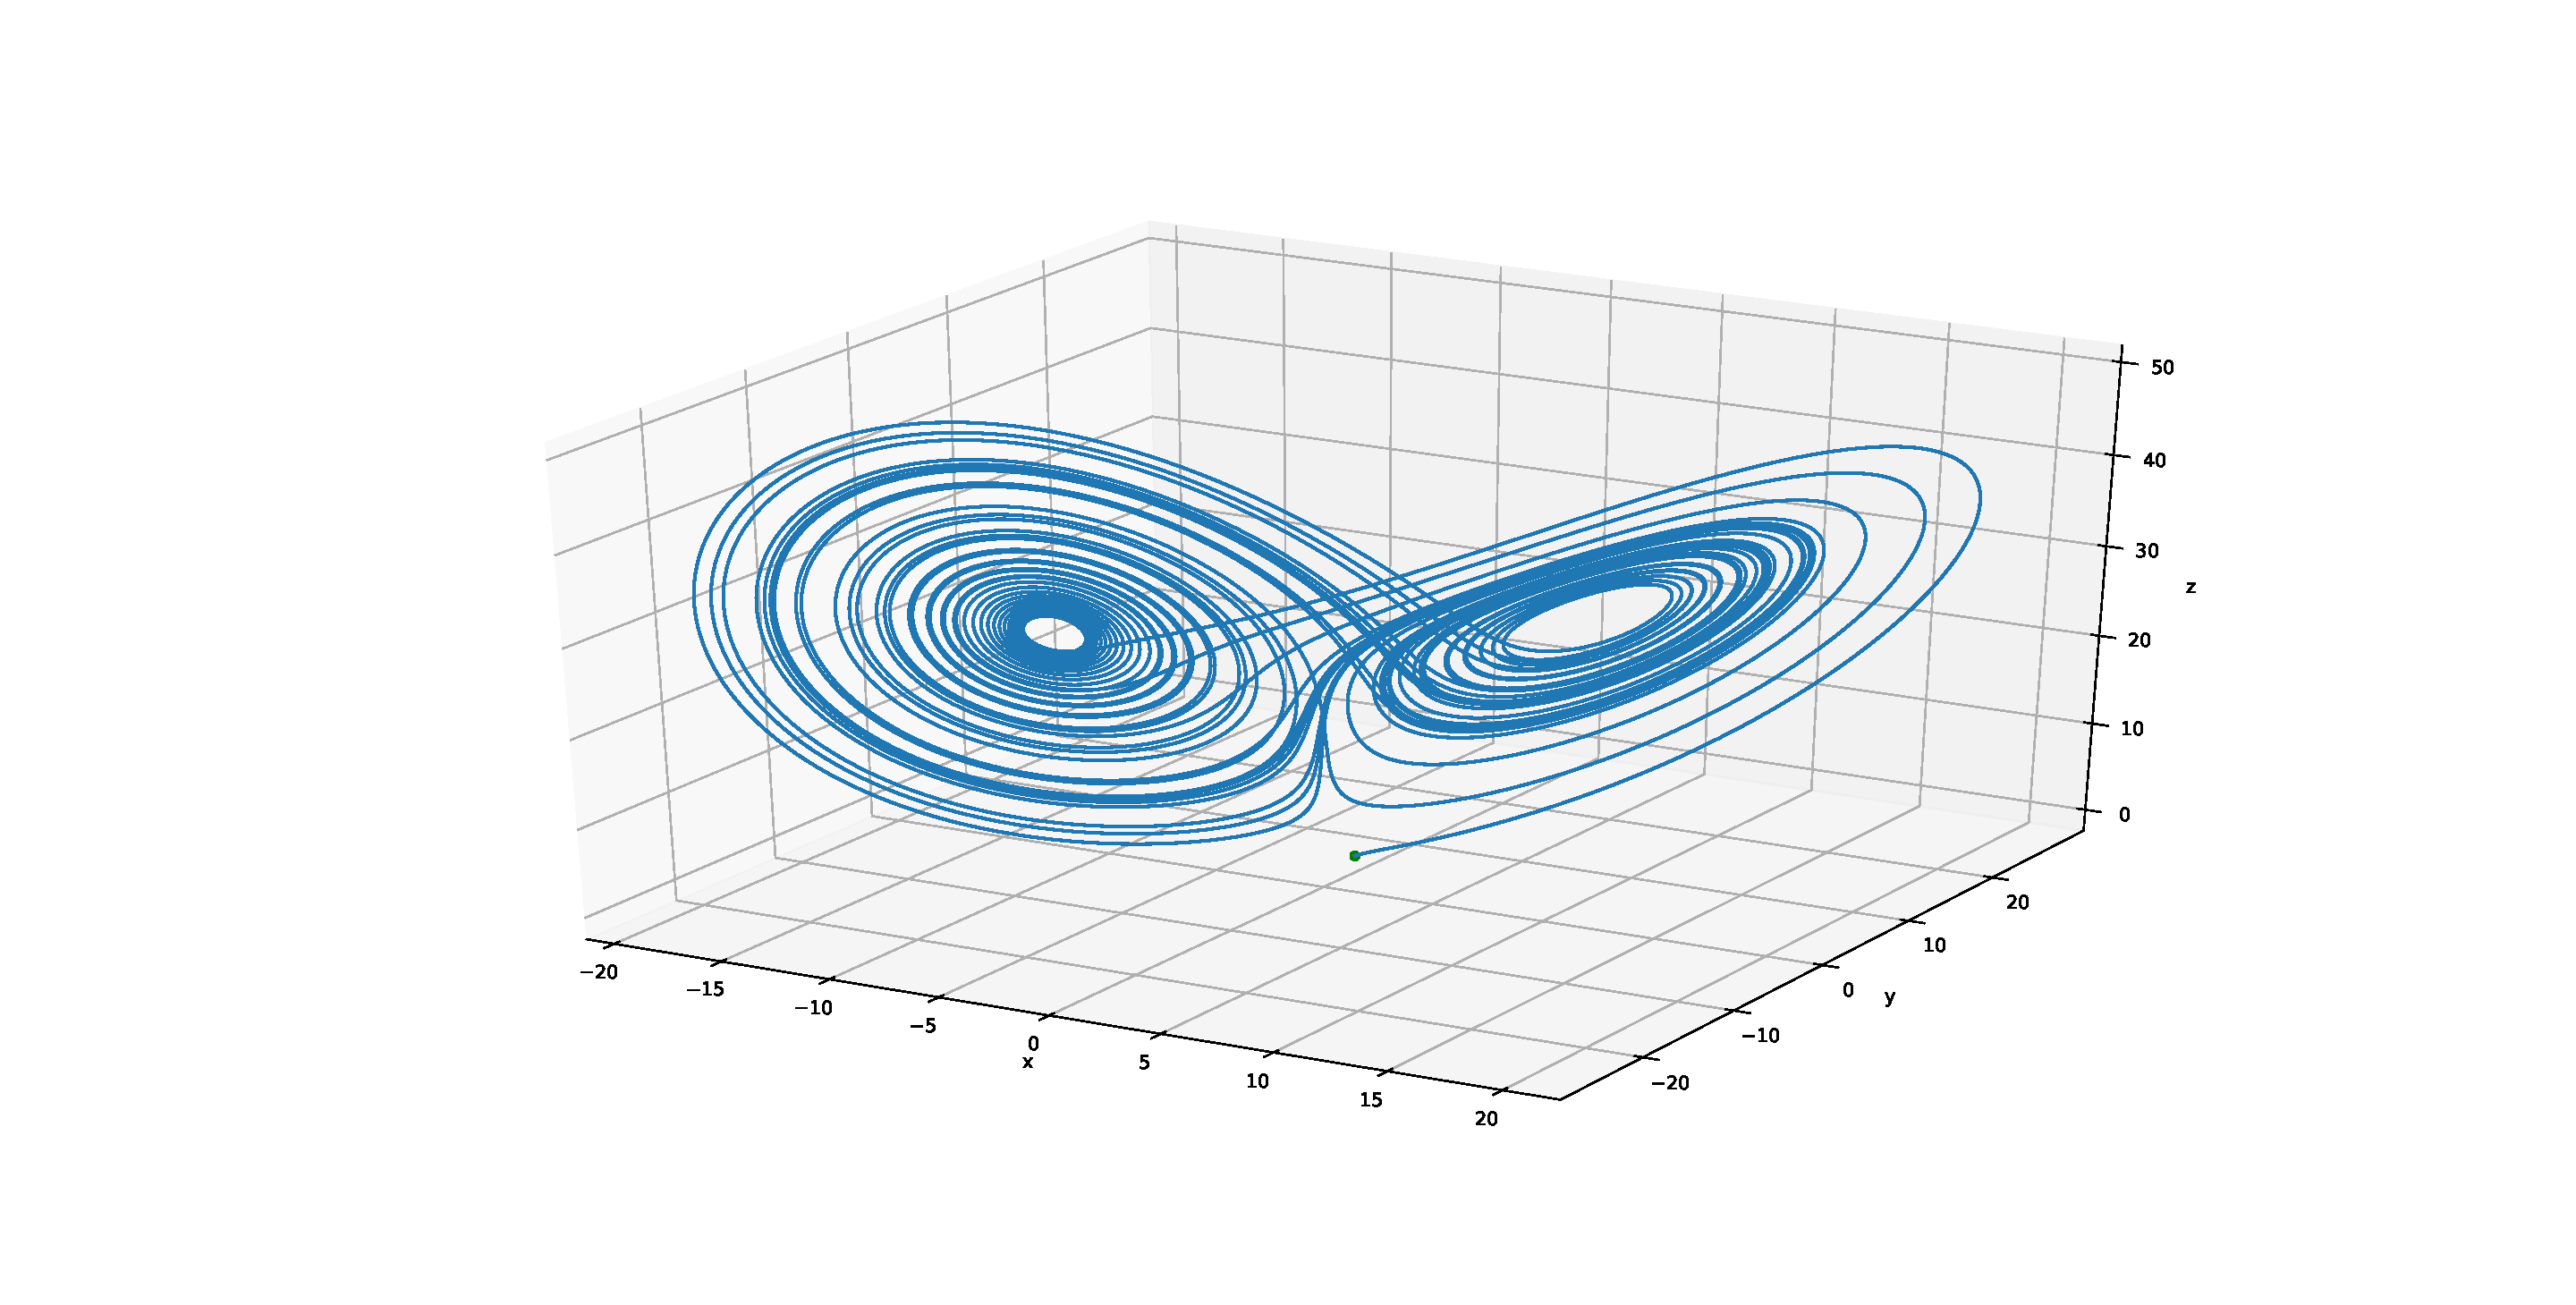
\includegraphics[width=0.75\textwidth]{figures/q2-3d-trajectory}
    \caption{Realization of a 50 seconds simulated trajectory. The initial
    position is indicated by the green dot. The resulting trajectory is chaotic
    (as expected for this set of paramaters).}
    \label{fig:q2-3d-trajectory}
\end{figure}

The trajectory of the first coordinates and the corresponding noisy measurements
are represented in figure~\ref{fig:q2-mes-vs-real}.

\begin{figure}[ht]
    \centering
    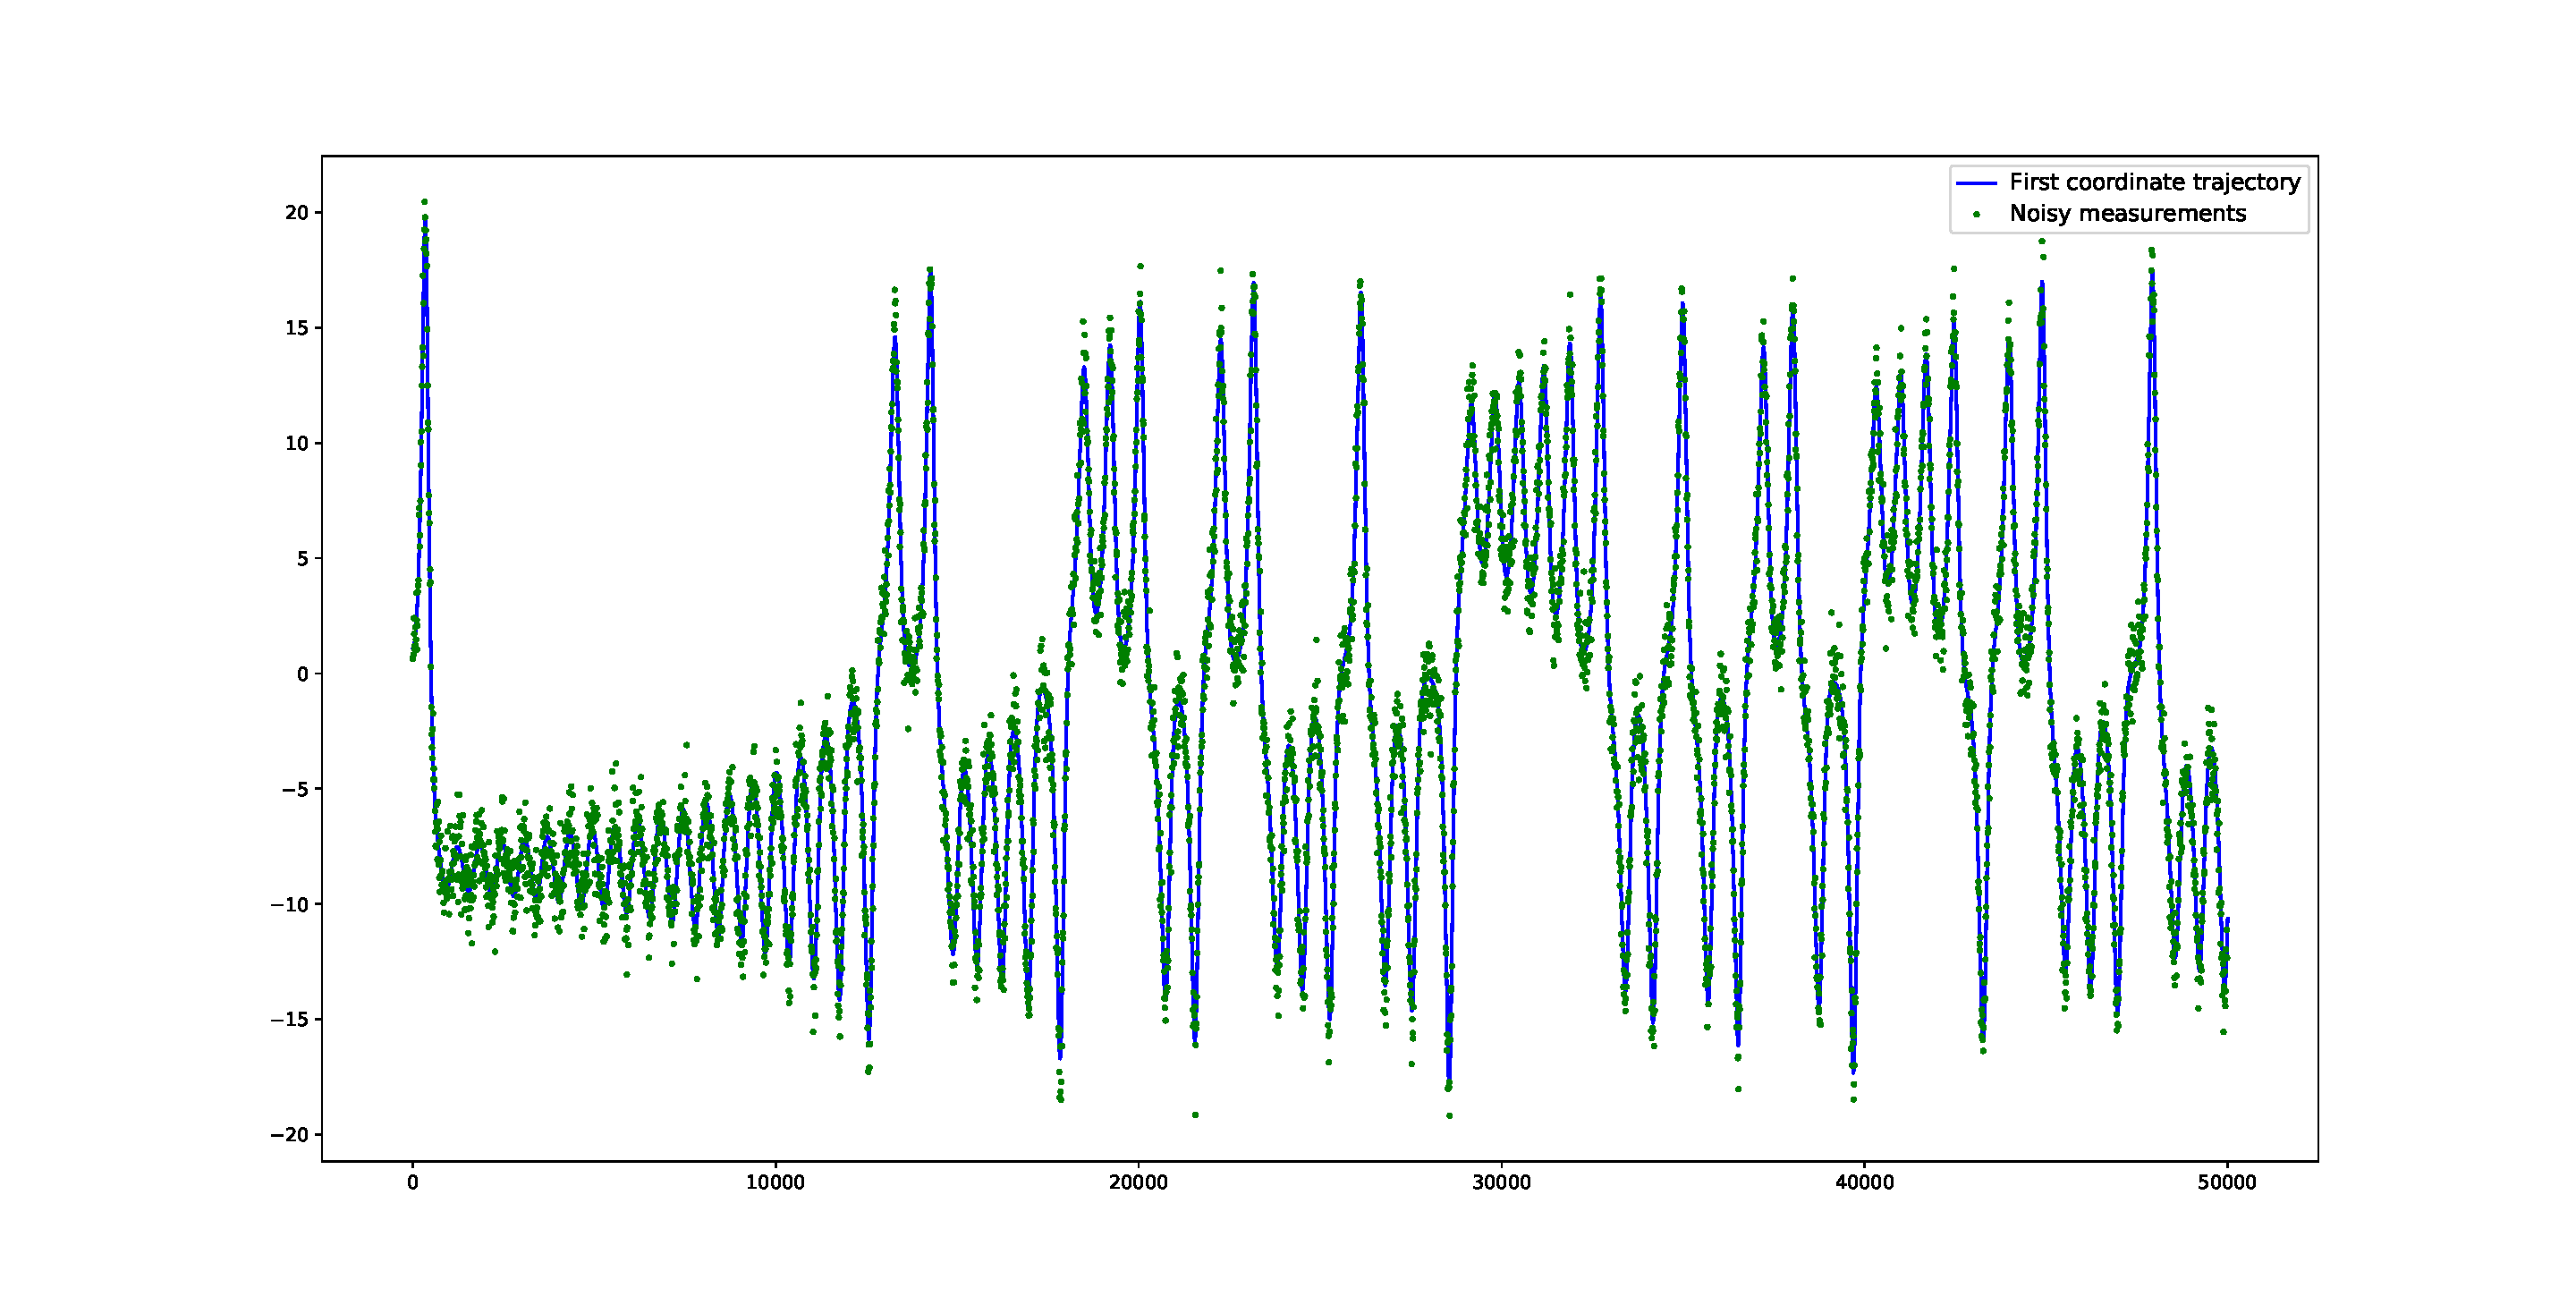
\includegraphics[width=0.75\textwidth]{figures/q2-mes-vs-real}
    \caption{Trajectory of the first coordinates and corresponding noisy measurements.}
    \label{fig:q2-mes-vs-real}
\end{figure}
\end{document}
